Utilizzando  GWT-RPC  tutte  le  chiamate  effettuate  dalla  pagina  HTML  al  server 
sono  asincrone.
Questo  significa  che  le  chiamate  non  bloccano  il  client  mentre attende   una 
risposta   dal   server,   ma   viene  eseguito   il   codice   immediatamente 
successivo.

\begin{figure}[!htb]
\centering%
\includegraphics[scale=0.5]{AnatomySVG.png}%
\caption{GWT-RPC }\label{fig:GWT-RPC}%
\end{figure}

\section*{Database}
L'applicazione usa come supporto un database contenente i dati rigurdanti le aule dei vari edifici universitari e del personale.
\`E fondamentale però mettere in evidenza con un adeguato schema Entità / Relazione le 
tabelle utilizzate all’interno del progetto e create al fine del corretto funzionamento del 
sistema.

\begin{figure}[!htb]
\centering
\includegraphics[scale=0.55]{databaseER.png}
\caption{Diagramma E/R del database}\label{fig:database}
\end{figure}
\begin{figure}[!htb]
\centering
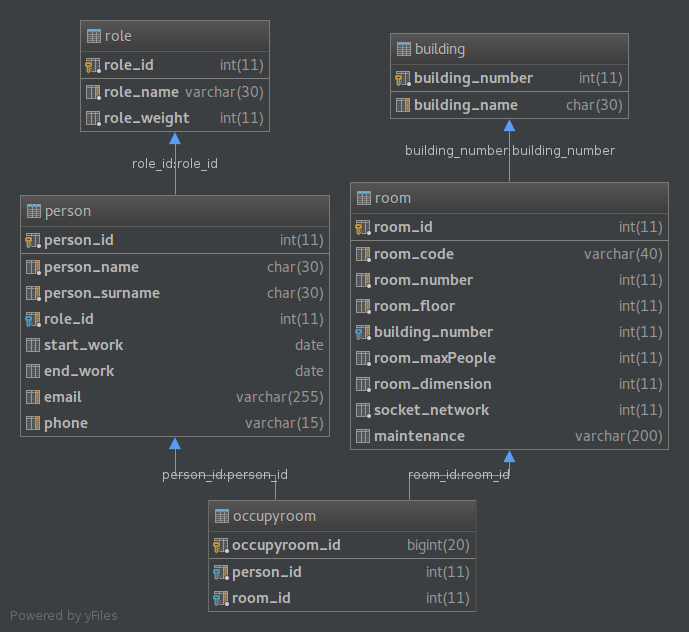
\includegraphics[scale=0.55]{diagram.png}
\caption{Schema Relazionale del database}\label{fig:databaseSchema}
\end{figure}